% =====================================================================
%  Informe - Big Data (Universidad ESAN)
%  Predicción de exposición y vulnerabilidad sísmica de edificaciones
%  Compilar con pdfLaTeX (Overleaf: Menu -> Compiler -> pdfLaTeX)
% =====================================================================
\IfFileExists{IEEEtran.cls}{%
  \documentclass[conference]{IEEEtran}%
}{%
  % Respaldo solo para compilar fuera de Overleaf si falta IEEEtran
  \documentclass[10pt,twocolumn,a4paper]{article}%
  \usepackage[margin=1.8cm]{geometry}%
}
% Equivalencias mínimas si no se usa IEEEtran (no afectan a IEEEtran)
\providecommand{\IEEEauthorblockN}[1]{\begin{tabular}{@{}c@{}}\textbf{#1}\end{tabular}\\}
\providecommand{\IEEEauthorblockA}[1]{\begin{tabular}{@{}c@{}}\small #1\end{tabular}}
\makeatletter
\@ifundefined{IEEEkeywords}{%
  \newenvironment{IEEEkeywords}{\par\noindent\textbf{\textit{Palabras clave}---}\bfseries}{\par}}{}
\makeatother

\usepackage[T1]{fontenc}
\usepackage[utf8]{inputenc}
\IfFileExists{spanish.ldf}{%
  \usepackage[spanish,es-tabla,es-nodecimaldot]{babel}%
}{%
  \usepackage{babel}\babelprovide[import,main]{spanish}%
  \setlocalecaption{spanish}{table}{Tabla}%
}
\usepackage{amsmath,amssymb}
\usepackage{graphicx}
\usepackage{booktabs}
\usepackage{tabularx}
\usepackage{multirow}
\usepackage{makecell}
\usepackage{array}
\usepackage[table]{xcolor}
\usepackage{tikz}
\usetikzlibrary{arrows.meta,positioning,fit,backgrounds,calc,shapes.geometric}
\usepackage{url}
\usepackage[hidelinks]{hyperref}
\usepackage{caption}
\captionsetup{font=footnotesize,labelsep=period}

\graphicspath{{figuras/}}
\newcolumntype{Y}{>{\raggedright\arraybackslash}X}
\newcommand{\fuente}[1]{\par\vspace{2pt}{\footnotesize\textit{Fuente:} #1}}
\newcommand{\vs}{V_{s30}}
\providecommand{\IEEEkeywordsname}{}
\renewcommand{\IEEEkeywordsname}{Palabras clave}

\begin{document}

\title{Predicción de Exposición y Vulnerabilidad en Edificaciones ante Ondas Sísmicas mediante Imágenes Geo Satelitales, Topografía del Suelo y Big Data}

\author{
\IEEEauthorblockN{Quiliche Chávez Andrés}
\IEEEauthorblockA{Facultad de Ingeniería\\Universidad ESAN\\Lima, Perú\\22200144@ue.edu.pe}
\and
\IEEEauthorblockN{Vergara Marcos Eduardo Coli}
\IEEEauthorblockA{Facultad de Ingeniería\\Universidad ESAN\\Lima, Perú\\22200217@ue.edu.pe}
\and
\IEEEauthorblockN{Jehu Salazar Irrazabal}
\IEEEauthorblockA{Facultad de Ingeniería\\Universidad ESAN\\Lima, Perú\\23100873@ue.edu.pe}
\and
\IEEEauthorblockN{Tucto Magiliano Chayna}
\IEEEauthorblockA{Facultad de Ingeniería\\Universidad ESAN\\Lima, Perú\\23101292@ue.edu.pe}
}

\date{}
\maketitle

% ---------------------------------------------------------------------
\begin{abstract}
La alta actividad sísmica del territorio peruano, asociada a la subducción de la placa de Nazca bajo la placa Sudamericana, representa un riesgo permanente para la población y la infraestructura urbana de Lima Metropolitana. Ante un sismo, la onda no afecta por igual a todas las edificaciones: el suelo la amplifica según su rigidez y, cuando el periodo de vibración del edificio se acerca al periodo del suelo, se produce resonancia y la demanda estructural crece. En este trabajo se propone un sistema de estimación de exposición y vulnerabilidad física por edificio, construido sobre una arquitectura \emph{lakehouse} de tipo medallón (Bronze, Silver y Gold) en Apache Spark y Delta Lake. El sistema integra 11 fuentes heterogéneas (${\sim}55$~GB): acelerogramas reales de Lima de la red del CISMID, el mapa de $\vs$ del USGS, la microzonificación sísmica de Lima, 7.2 millones de huellas de edificaciones extraídas de imágenes satelitales (Google Open Buildings) y su altura (Open Buildings 2.5D), la Norma E.030, y datos de validación del sismo de Turquía de 2023 (imágenes Maxar, ShakeMap del USGS y el conjunto xBD). A partir de cada registro se calcula el espectro de respuesta $S_a(T)$; con las propias ondas de Lima se mide la amplificación del suelo mediante un modelo Random Forest en Spark MLlib; y se estima la demanda $S_a(T_b)$ y la probabilidad de daño de 1.92 millones de edificaciones mediante curvas de fragilidad, clasificándolas en niveles de riesgo bajo, medio y alto. La propuesta incorpora además un flujo en tiempo real con Apache Kafka y Spark Structured Streaming, y un tablero geoespacial para la gestión del riesgo de desastres.
\end{abstract}

\begin{IEEEkeywords}
Big Data, Apache Spark, Delta Lake, arquitectura medallón, riesgo sísmico, amplificación del suelo, $V_{s30}$, espectro de respuesta, curvas de fragilidad, imágenes satelitales, Lima Metropolitana.
\end{IEEEkeywords}

% =====================================================================
\section{Introducción}
% =====================================================================
El Perú presenta una elevada actividad sísmica debido a la convergencia de la placa de Nazca bajo la placa Sudamericana, proceso que en el margen occidental peruano ocurre a una velocidad aproximada de 7--8~cm/año. Debido a este proceso, el Instituto Geofísico del Perú (IGP) registra aproximadamente 800 sismos percibidos por la población cada año \cite{tavera2024}. Además, los sismos de magnitud $M \geq 7.0$ pueden generar niveles elevados de sacudimiento en áreas extensas; por ejemplo, el sismo de Yauca del 28 de junio de 2024, de $M7.0$ y 42~km de profundidad, fue percibido hasta aproximadamente 500~km del epicentro \cite{tavera2024}.

Lima Metropolitana concentra una población proyectada de 10\,432\,133 habitantes, lo que incrementa sustancialmente la exposición física y social ante eventos sísmicos \cite{inei2025}. Esta exposición no es uniforme y depende de la interacción entre las ondas sísmicas, las características del suelo y la calidad de las construcciones. Por ejemplo, el 15 de junio de 2025, un sismo de $M6.1$ con epicentro a 30~km al suroeste del Callao y 49~km de profundidad produjo en Lima Metropolitana y el Callao aceleraciones del suelo ($PGA$) de entre 50 y 100~cm/s$^2$, con máximos de 251~cm/s$^2$ en Villa María del Triunfo, 198~cm/s$^2$ en San Juan de Miraflores y 192~cm/s$^2$ en Villa El Salvador \cite{tavera2025}. Estos valores muestran que el suelo local amplifica la energía de la onda de forma heterogénea en la ciudad.

Actualmente, el Sistema de Alerta Sísmica Peruano (SASPe) cuenta con 106 estaciones acelerométricas y una cobertura estimada de 18\,363\,626 ciudadanos, 76 provincias, 669 distritos y 10 regiones, con el objetivo de emitir alertas ante sismos potencialmente peligrosos \cite{igp_saspe}. Sin embargo, las alertas convencionales emiten avisos generales que no determinan el nivel de exposición física ni el grado de daño potencial que sufrirán las edificaciones de una zona específica según la respuesta de su suelo.

En este contexto, el presente estudio propone un sistema distribuido en \textbf{Apache Spark} que combina procesamiento de señales, análisis geoespacial y \textbf{Machine Learning} para predecir la exposición y vulnerabilidad de cada edificación de Lima Metropolitana ante la propagación de ondas sísmicas. La propuesta integra la \textbf{huella y altura de las edificaciones} extraídas de imágenes satelitales, la \textbf{respuesta del suelo} ($\vs$, periodo del suelo y microzonificación) y los \textbf{registros reales de la onda sísmica} (espectro de respuesta, $PGA$ y periodo predominante). El resultado es un mapa que clasifica el riesgo de cada edificación en niveles \emph{bajo, medio y alto}, útil para focalizar alertas y priorizar la respuesta ante emergencias.

La pregunta de investigación es: \emph{¿qué edificaciones de Lima serán más afectadas por un sismo, según cómo el suelo amplifica la onda y si el edificio entra en resonancia con ella?} La hipótesis es que las edificaciones sobre suelos blandos (bajo $\vs$), cuyo periodo de vibración $T_b$ se acerca al periodo del suelo $T_P$, reciben mayor demanda sísmica y presentan mayor probabilidad de daño.

El resto del documento se organiza así: la Sección~\ref{sec:estado} revisa seis trabajos relacionados; la Sección~\ref{sec:propuesta} describe la propuesta metodológica, las bases de datos y las tecnologías de Big Data; y la Sección~\ref{sec:conclusiones} resume los aportes esperados.

% =====================================================================
\section{Estado del arte}\label{sec:estado}
% =====================================================================
Se revisaron seis trabajos que abordan, desde distintos ángulos, los componentes del sistema propuesto: la extracción automática de características de edificaciones a partir de imágenes \cite{carpanese2023}, la estimación de la vulnerabilidad sísmica con teledetección y aprendizaje automático \cite{fan2021plsv}, la evaluación de daño con imágenes satelitales antes y después de un desastre \cite{gupta2019xbd}, y el procesamiento escalable de ondas sísmicas en lote y en tiempo real \cite{zhu2022quakeflow,li2022yangbi,xiao2026edge}. La Tabla~\ref{tab:comparativa} resume la comparación.

% ---------------------------------------------------------------------
\subsection{Automatic identification of residential building features using machine learning techniques (Carpanese et al., 2023)}

\textbf{Problema:} La evaluación de la vulnerabilidad sísmica de edificaciones requiere información detallada sobre sus características constructivas. Recopilarla mediante inspecciones de campo demanda una considerable inversión de tiempo y recursos, especialmente cuando se analiza un gran número de edificaciones. Por ello, los autores investigan cómo identificar automáticamente características relevantes de edificios residenciales a partir de imágenes, para facilitar evaluaciones de vulnerabilidad a mayor escala \cite{carpanese2023}.

\textbf{Base de datos:} El estudio utiliza \textbf{imágenes satelitales e imágenes de Google Street View} de edificaciones residenciales de Pordenone (Italia), complementadas con cartografía abierta de edificios. Las imágenes son la fuente para identificar atributos que luego alimentan la evaluación de vulnerabilidad sísmica.

\textbf{Técnicas y tecnologías:} Combina \textbf{visión por computadora} y \textbf{aprendizaje automático}. Las imágenes satelitales aportan la ubicación y configuración de los edificios, y las de Street View, las características visibles de las fachadas (Fig.~\ref{fig:carp_flujo}).
\begin{itemize}
  \item \textbf{Visión por computadora:} uso de imágenes de sensores remotos y Street View como fuente visual, sin depender exclusivamente de inspecciones presenciales (Fig.~\ref{fig:carp_deteccion}).
  \item \textbf{Aprendizaje automático:} modelos que clasifican altura, material y periodo de construcción de cada edificio (Fig.~\ref{fig:carp_ml}).
  \item \textbf{Extracción automatizada de características:} transformación de la información visual en atributos utilizables para caracterizar el comportamiento sísmico.
\end{itemize}

\begin{figure}[!t]
\centering
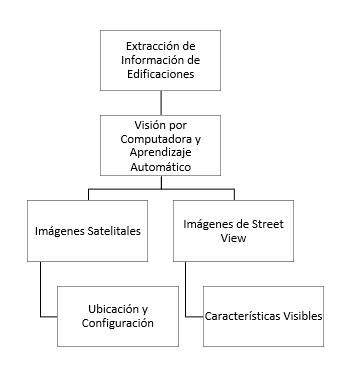
\includegraphics[width=0.62\columnwidth]{image1.png}
\caption{Flujo metodológico para la extracción de información de edificaciones mediante visión por computadora e imágenes multifuente (satelital y Street View).}
\label{fig:carp_flujo}
\fuente{Elaboración propia a partir de Carpanese et al. \cite{carpanese2023}.}
\end{figure}

\begin{figure}[!t]
\centering
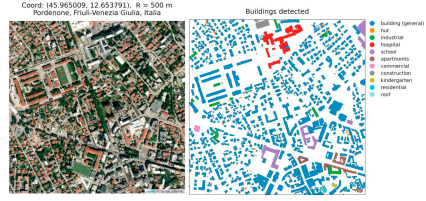
\includegraphics[width=\columnwidth]{image5.png}\\[2pt]
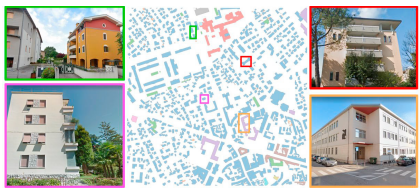
\includegraphics[width=\columnwidth]{image12.png}
\caption{Identificación automática de edificaciones: detección sobre imagen satelital (arriba) y asociación con imágenes de Street View (abajo).}
\label{fig:carp_deteccion}
\fuente{Adaptado de Carpanese, Donà y da Porto \cite{carpanese2023}.}
\end{figure}

\begin{figure}[!t]
\centering
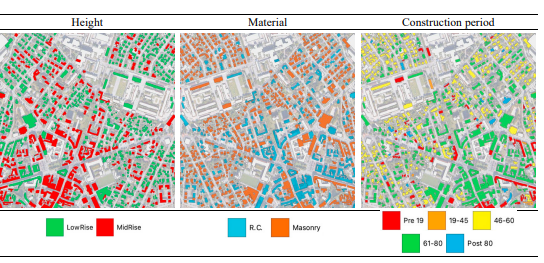
\includegraphics[width=\columnwidth]{image14.png}
\caption{Clasificación automática de altura, material y periodo de construcción de edificaciones mediante aprendizaje automático.}
\label{fig:carp_ml}
\fuente{Carpanese et al. \cite{carpanese2023}.}
\end{figure}

\textbf{Metodología:} Primero se emplean imágenes satelitales para obtener la información espacial de las edificaciones; luego, imágenes de Street View para obtener características visuales adicionales; finalmente, los modelos de Machine Learning procesan ambas fuentes para identificar automáticamente los atributos relevantes para la evaluación de vulnerabilidad sísmica.

\textbf{Resultados:} Los autores muestran que es posible usar aprendizaje automático con imágenes obtenidas remotamente para identificar características de edificios residenciales, reduciendo la necesidad de inspecciones presenciales y facilitando la recopilación de información para estudios de vulnerabilidad sobre un mayor número de edificaciones.

\textbf{Aporte a la investigación:} Demuestra la viabilidad de obtener automáticamente, a partir de imágenes, atributos de las edificaciones relacionados con su vulnerabilidad. En este proyecto el enfoque se amplía integrando huellas y alturas derivadas de imágenes satelitales con datos del suelo y registros sísmicos reales, procesados con tecnologías de Big Data a escala metropolitana.

% ---------------------------------------------------------------------
\subsection{Estimation of pixel-level seismic vulnerability of the building environment based on mid-resolution optical remote sensing images (Fan et al., 2021)}

\textbf{Problema:} Evaluar la vulnerabilidad sísmica de las edificaciones en áreas extensas es costoso, porque los métodos tradicionales dependen de inspecciones de campo edificio por edificio. Además, interpolar espacialmente los puntos inspeccionados no captura bien la heterogeneidad del entorno construido. Los autores proponen estimar la \emph{vulnerabilidad sísmica a nivel de píxel} (PLSV) del entorno construido a partir de imágenes satelitales de resolución media y aprendizaje automático \cite{fan2021plsv}.

\textbf{Base de datos:} El estudio se realizó en la ciudad de Yancheng (provincia de Jiangsu, China), con ubicaciones de investigación de campo distribuidas por sus condados (Fig.~\ref{fig:fan_area}), que sirven como verdad de terreno. Como variables predictoras integra datos multifuente de teledetección: luces nocturnas VIIRS, índice de vegetación y reflectancia de superficie MODIS, y texturas derivadas de la reflectancia de superficie de Landsat-8 OLI.

\begin{figure}[!t]
\centering
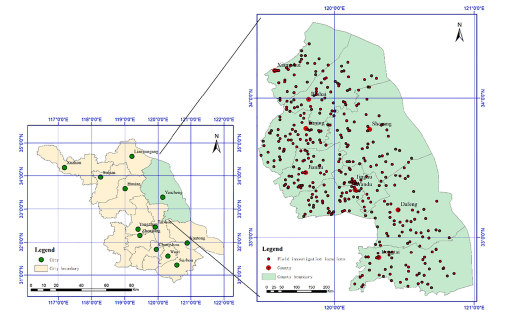
\includegraphics[width=\columnwidth]{yancheng_area.png}
\caption{Área de estudio: ubicación de Yancheng en la provincia de Jiangsu y puntos de investigación de campo.}
\label{fig:fan_area}
\fuente{Fan et al. \cite{fan2021plsv}.}
\end{figure}

\textbf{Técnicas y tecnologías:}
\begin{itemize}
  \item \textbf{Teledetección multifuente:} VIIRS (actividad humana), MODIS (vegetación y reflectancia) y Landsat-8 OLI (textura del entorno construido).
  \item \textbf{Regresión por vectores de soporte (SVR)} y \textbf{Random Forest}: modelos que relacionan las variables satelitales con la vulnerabilidad observada en campo.
  \item \textbf{Interpolación espacial:} método de referencia para comparar con los modelos de aprendizaje automático.
  \item \textbf{SIG:} integración de las capas en una grilla de píxeles y elaboración de mapas.
\end{itemize}

\textbf{Metodología:} (1) se calcula la vulnerabilidad sísmica de las edificaciones inspeccionadas en campo; (2) se extraen, para cada píxel, las variables de luces nocturnas, vegetación, reflectancia y textura; (3) se dividen los puntos en entrenamiento y prueba; (4) se entrenan SVR y Random Forest para predecir la PLSV; y (5) se compara su error con el de la interpolación espacial y se genera el mapa de PLSV de toda la ciudad (Fig.~\ref{fig:fan_plsv}).

\begin{figure}[!t]
\centering
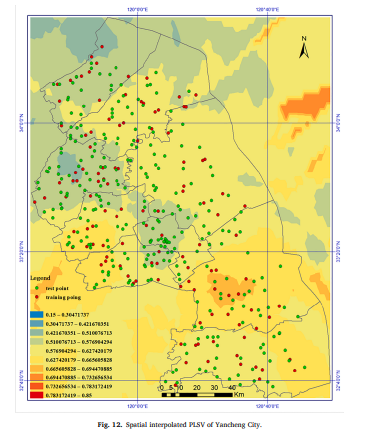
\includegraphics[width=0.85\columnwidth]{yancheng_plsv.png}
\caption{PLSV de Yancheng obtenida por interpolación espacial, con los puntos de entrenamiento (rojo) y de prueba (verde).}
\label{fig:fan_plsv}
\fuente{Fan et al. \cite{fan2021plsv}.}
\end{figure}

\textbf{Resultados:} El enfoque basado en imágenes satelitales y aprendizaje automático estimó la PLSV con un error cuadrático medio (RMSE) de aproximadamente 0.1, superando a los métodos convencionales de interpolación espacial. Esto demuestra que la vulnerabilidad del entorno construido puede cartografiarse a escala urbana con datos satelitales abiertos y un número limitado de inspecciones de campo.

\textbf{Aporte a la investigación:} Es el antecedente más cercano a este proyecto: estima vulnerabilidad sísmica con imágenes satelitales y Random Forest, y muestra que el aprendizaje automático supera a la interpolación espacial. Este proyecto avanza un paso más al incorporar la onda sísmica registrada y la respuesta del suelo, para pasar de una vulnerabilidad estática a la demanda y el daño esperados ante un sismo concreto.

% ---------------------------------------------------------------------
\subsection{xBD: A Dataset for Assessing Building Damage from Satellite Imagery (Gupta et al., 2019)}

\textbf{Problema:} Tras un desastre, la respuesta humanitaria necesita saber con rapidez qué edificaciones resultaron dañadas. Las evaluaciones presenciales demoran entre 24 y 48~horas y exponen al personal a riesgos. Aunque la visión por computadora sobre imágenes aéreas podría acelerar el proceso, no existía un conjunto de datos público, grande y estandarizado de imágenes antes y después del evento con daño etiquetado por edificio \cite{gupta2019xbd}.

\textbf{Base de datos:} xBD contiene imágenes satelitales de alta resolución (menos de 0.8~m por píxel) del programa Maxar Open Data para 19 desastres naturales (sismos, tsunamis, huracanes, inundaciones, incendios y erupciones). Reúne 22\,068 imágenes, 45\,362~km$^2$ y 850\,736 polígonos de edificaciones, cada uno con su nivel de daño en la escala conjunta \emph{Joint Damage Scale}: sin daño, daño leve, daño severo y destruido.

\textbf{Técnicas y tecnologías:}
\begin{itemize}
  \item \textbf{Anotación a gran escala:} digitalización de polígonos sobre la imagen previa y clasificación del daño sobre la posterior, revisada por expertos (con una tasa de corrección de 2--3\,\%).
  \item \textbf{U-Net:} segmentación semántica para localizar edificaciones.
  \item \textbf{ResNet-50 + CNN:} clasificación del nivel de daño de cada edificio.
  \item \textbf{Partición 80/10/10} para entrenamiento, prueba y retención, y base del concurso xView2.
\end{itemize}

\textbf{Metodología:} El flujo consta de cuatro etapas (Fig.~\ref{fig:xbd}): selección de eventos e imágenes, anotación de edificios sobre la imagen previa, etiquetado del daño sobre la imagen posterior y entrenamiento de modelos de referencia en dos tareas, localización y clasificación del daño.

\begin{figure}[!t]
\centering
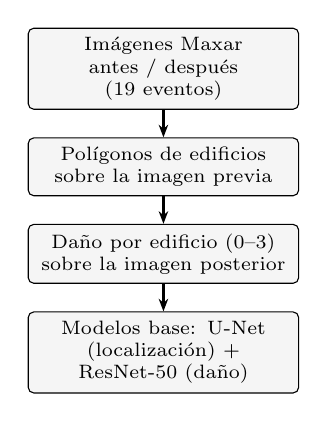
\begin{tikzpicture}[
  node distance=3.5mm,
  caja/.style={draw, rounded corners=2pt, align=center, font=\scriptsize, minimum height=7mm, text width=3.2cm, fill=gray!8},
  flecha/.style={-{Stealth[length=1.6mm]}, thick}]
\node[caja] (a) {Imágenes Maxar\\antes / después (19 eventos)};
\node[caja, below=of a] (b) {Polígonos de edificios\\sobre la imagen previa};
\node[caja, below=of b] (c) {Daño por edificio (0--3)\\sobre la imagen posterior};
\node[caja, below=of c] (d) {Modelos base: U-Net\\(localización) + ResNet-50 (daño)};
\draw[flecha] (a) -- (b); \draw[flecha] (b) -- (c); \draw[flecha] (c) -- (d);
\end{tikzpicture}
\caption{Flujo de construcción del conjunto xBD y de sus modelos de referencia.}
\label{fig:xbd}
\fuente{Elaboración propia a partir de Gupta et al. \cite{gupta2019xbd}.}
\end{figure}

\textbf{Resultados:} El modelo de localización alcanzó un IoU de 0.66 para edificios y 0.97 para el fondo. El clasificador de daño obtuvo un F1 ponderado de 0.2654, con F1 de 0.6631 para \emph{sin daño}, 0.1435 para \emph{leve}, 0.0094 para \emph{severo} y 0.4657 para \emph{destruido}. Estos valores evidencian la dificultad de distinguir los niveles intermedios de daño.

\textbf{Aporte a la investigación:} xBD se utiliza para entrenar la red U-Net siamesa con la que se medirá el daño real del sismo de Turquía de 2023 y se validará la cadena predictiva propuesta.

% ---------------------------------------------------------------------
\subsection{QuakeFlow: A Scalable Machine-learning-based Earthquake Monitoring Workflow with Cloud Computing (Zhu et al., 2022)}

\textbf{Problema:} El incremento de redes sísmicas densas y la adquisición continua de formas de onda han producido volúmenes masivos de datos que los flujos convencionales no procesan con eficiencia. En abril de 2022, el archivo sísmico de IRIS alcanzaba aproximadamente 800~TiB, y tecnologías como \emph{Distributed Acoustic Sensing} aumentan aún más la tasa de generación de datos \cite{zhu2022quakeflow}.

\textbf{Base de datos:} Se procesaron tres años de registros continuos de Puerto Rico (1 de mayo de 2018 al 1 de mayo de 2021), correspondientes a 70 estaciones y unos 210 años-estación de datos tricomponentes de la Puerto Rico Seismic Network y redes del USGS. Además, se usaron registros de 66 estaciones del Hawaiian Volcano Observatory.

\textbf{Técnicas y tecnologías de Big Data:}
\begin{itemize}
  \item \textbf{Apache Kafka:} transmisión distribuida de formas de onda.
  \item \textbf{Apache Spark Streaming:} procesamiento ETL en tiempo real en ventanas de 30~s.
  \item \textbf{Kubernetes:} contenedores, autoescalado y procesamiento paralelo en la nube.
  \item \textbf{PhaseNet (CNN):} identificación de las fases sísmicas P y S.
  \item \textbf{GaMMA (modelo de mezcla gaussiana):} asociación de fases y estimación de ubicación y magnitud.
\end{itemize}

\textbf{Metodología:} El flujo (Fig.~\ref{fig:quakeflow}) descarga los datos de archivos sísmicos con ObsPy o los recibe en tiempo real mediante Kafka y Spark Streaming; detecta las fases con PhaseNet; las asocia con GaMMA; relocaliza los eventos con HypoDD y publica un catálogo y un monitoreo en tiempo real, todo desplegado en Kubernetes con reentrenamiento mediante Kubeflow.

\begin{figure}[!t]
\centering
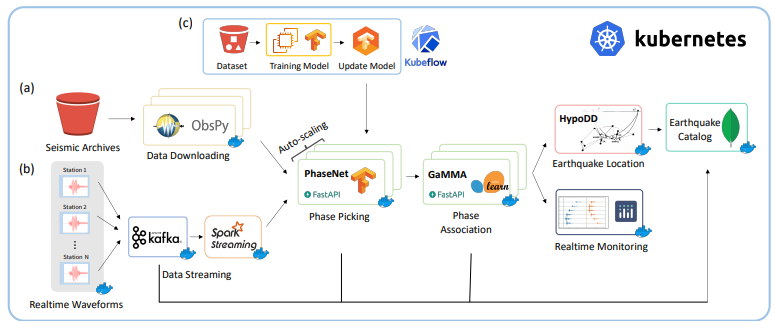
\includegraphics[width=\columnwidth]{image8.png}
\caption{Arquitectura de QuakeFlow: (a) procesamiento de archivos históricos, (b) flujo en tiempo real con Kafka y Spark Streaming y (c) actualización de modelos, sobre Kubernetes.}
\label{fig:quakeflow}
\fuente{Zhu et al. \cite{zhu2022quakeflow}.}
\end{figure}

\textbf{Resultados:}
\begin{itemize}
  \item 143\,704 eventos detectados en Puerto Rico frente a 18\,041 del catálogo convencional ($7.97\times$).
  \item 81\,284 eventos en Hawái frente a 7\,761 del catálogo estándar ($10.47\times$), con una imagen detallada de la estructura sísmica bajo los volcanes (Fig.~\ref{fig:quakeflow_res}).
  \item Tiempo de procesamiento: 3.5~h de descarga, 3~h de PhaseNet y 0.5~h de GaMMA.
\end{itemize}

\begin{figure}[!t]
\centering
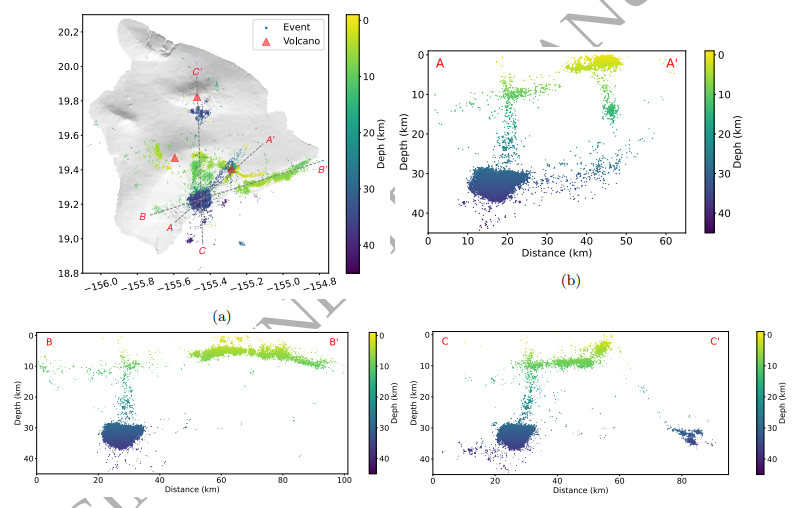
\includegraphics[width=\columnwidth]{image10.png}
\caption{Sismicidad de Hawái detectada por QuakeFlow: (a) mapa de eventos y (b)--(d) perfiles de profundidad.}
\label{fig:quakeflow_res}
\fuente{Zhu et al. \cite{zhu2022quakeflow}.}
\end{figure}

\textbf{Aporte a la investigación:} Valida el uso combinado de Kafka y Spark Streaming para procesar formas de onda en tiempo real, que este proyecto adopta para su módulo de velocidad.

% ---------------------------------------------------------------------
\subsection{A real-time AI-assisted seismic monitoring system based on new nodal stations with 4G telemetry and its application in the Yangbi MS 6.4 aftershock monitoring in southwest China (Li et al., 2022)}

\textbf{Problema:} Las redes sísmicas permanentes tienen limitaciones para detectar eventos de baja magnitud y para transmitir en tiempo real los datos de estaciones nodales. El procesamiento manual de formas de onda continuas incrementa además el tiempo requerido para detectar, localizar y caracterizar los eventos \cite{li2022yangbi}.

\textbf{Base de datos:} Registros de una red temporal de 15 estaciones nodales UGL-4G de tres componentes, desplegada para monitorear las réplicas del sismo de Yangbi ($M_S$~6.4) del 21 de mayo de 2021, entre el 27 de mayo y el 17 de junio de 2021. Como referencia se empleó el catálogo del China Earthquake Networks Center (CENC).

\textbf{Técnicas y tecnologías:}
\begin{itemize}
  \item \textbf{Telemetría 4G:} transmisión de datos sísmicos con retraso inferior a 1~s.
  \item \textbf{U-Net:} detección de eventos y lectura de fases P y S.
  \item \textbf{NonLinLoc:} localización de los eventos.
  \item \textbf{Ajuste de forma de onda completa:} determinación del mecanismo focal.
\end{itemize}

\textbf{Metodología:} El flujo continuo de datos pasa por detección de eventos y lectura de fases asistidas por IA, localización de la fuente y cálculo de magnitud; si la magnitud supera un umbral, se invierte el mecanismo focal y se publican los atributos del evento (Fig.~\ref{fig:yangbi_flujo}). Los resultados se muestran en una plataforma web en tiempo real (Fig.~\ref{fig:yangbi_web}).

\begin{figure}[!t]
\centering
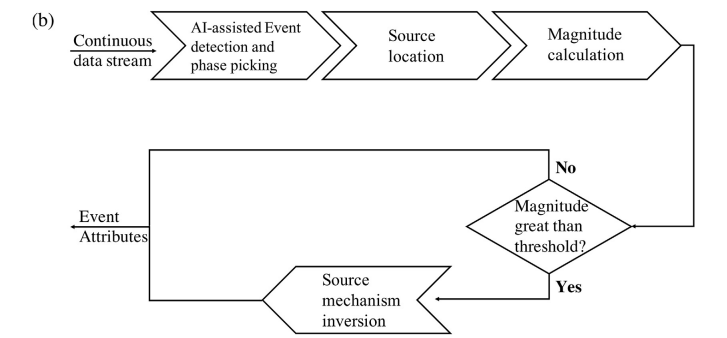
\includegraphics[width=\columnwidth]{image7.png}
\caption{Flujo de procesamiento en tiempo real asistido por IA.}
\label{fig:yangbi_flujo}
\fuente{Li et al. \cite{li2022yangbi}.}
\end{figure}

\textbf{Resultados:}
\begin{itemize}
  \item 7\,905 réplicas detectadas y localizadas durante el monitoreo.
  \item En 12 días, 6\,092 eventos detectados automáticamente frente a 1\,628 del catálogo del CENC.
  \item 6.5\,\% de falsas detecciones y 5.3\,\% de eventos no detectados.
  \item Magnitud de completitud de $M{-}0.1$ con la red temporal frente a $M0.2$ con la red permanente.
  \item Tiempo de procesamiento generalmente menor a un minuto.
  \item La mayor densidad de estaciones mejoró la estimación de profundidad y reveló una zona de falla previamente desconocida.
\end{itemize}

\begin{figure}[!t]
\centering
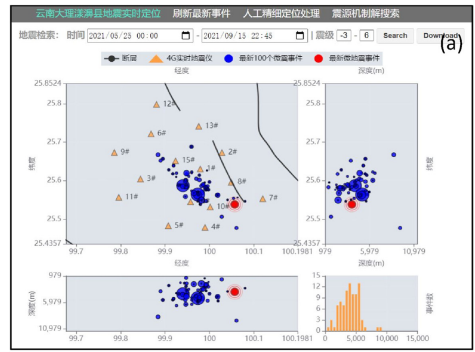
\includegraphics[width=0.92\columnwidth]{image2.png}
\caption{Plataforma web de localización en tiempo real de las réplicas de Yangbi.}
\label{fig:yangbi_web}
\fuente{Li et al. \cite{li2022yangbi}.}
\end{figure}

\textbf{Aporte a la investigación:} Muestra que una cadena automática de detección y caracterización de sismos puede entregar resultados en menos de un minuto, lo que respalda el componente de tiempo real de la propuesta.

% ---------------------------------------------------------------------
\subsection{Edge seismic phase picking: Model distillation for multimodal early-warning systems (Xiao et al., 2026)}

\textbf{Problema:} El crecimiento de redes sísmicas densas (arreglos MEMS, redes nodales y sistemas DAS) genera grandes volúmenes de datos que deben procesarse en tiempo real. Las arquitecturas centralizadas sufren limitaciones de ancho de banda, congestión y latencia, ya que deben enviar continuamente las formas de onda a servidores remotos antes de detectar las fases. Los autores proponen realizar la primera inferencia cerca del sensor mediante un modelo compacto de \emph{Edge Machine Learning} \cite{xiao2026edge}.

\textbf{Base de datos:} Cuatro conjuntos sísmicos: STEAD (${\sim}1.2$ millones de formas de onda de más de 450\,000 sismos), ETHZ (más de 20\,000 llegadas en Suiza y los Alpes), TXED (más de 20\,000 eventos y 200\,000 trazas de ruido) y OKLAD (más de un millón de trazas, usado para la destilación). Los registros se procesaron con SeisBench, se remuestrearon a 100~Hz y se dividieron en ventanas de 30~s, con una partición 70/15/15.

\textbf{Técnicas y tecnologías:}
\begin{itemize}
  \item \textbf{Destilación del conocimiento:} transferencia de un modelo grande (PhaseNet, \emph{teacher}) a uno compacto (XiaoNet, \emph{student}).
  \item \textbf{Arquitectura codificador-decodificador} con convoluciones separables en profundidad para reducir parámetros (Fig.~\ref{fig:xiaonet}).
  \item \textbf{SeisBench, PyTorch, ONNX y TensorRT:} acceso a datos y evaluación de modalidades de inferencia.
  \item \textbf{MQTT:} transmisión de solo los metadatos generados en el dispositivo.
\end{itemize}

\textbf{Metodología:} La forma de onda de tres canales atraviesa tres codificadores, un cuello de botella con un extractor multiescala (kernels de 3, 5 y 7) y tres decodificadores con conexiones residuales, hasta una capa de salida que entrega la probabilidad de onda P, onda S y ruido.

\begin{figure}[!t]
\centering
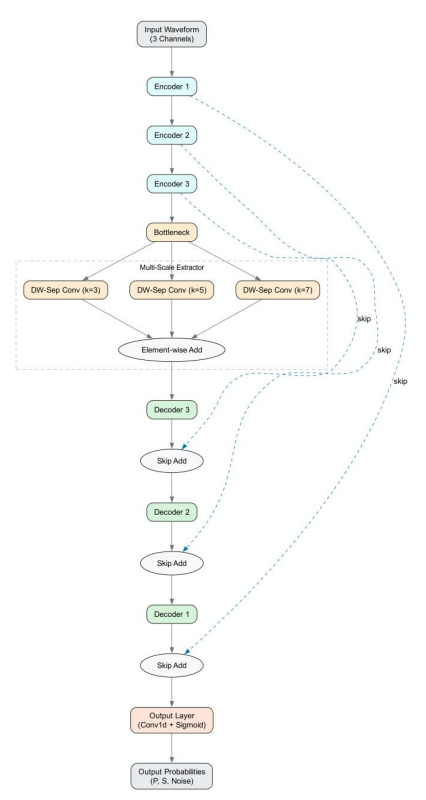
\includegraphics[width=0.55\columnwidth]{image4.png}
\caption{Arquitectura codificador-decodificador de XiaoNet para lectura de fases en el borde.}
\label{fig:xiaonet}
\fuente{Xiao et al. \cite{xiao2026edge}.}
\end{figure}

\textbf{Resultados:}
\begin{itemize}
  \item XiaoNet tiene 20\,208 parámetros entrenables y unos 240~KB, un 92.4\,\% menos que PhaseNet y un 94.6\,\% menos que EQTransformer.
  \item En STEAD, entrenado desde cero, alcanzó una tasa de verdaderos positivos de 95.58\,\% para la fase P y 94.67\,\% para la S; en ETHZ, 91.38\,\% para la P.
  \item Tras la destilación con el 100\,\% de OKLAD, logró F1~$=0.8629$ para P y F1~$=0.8610$ para S.
\end{itemize}

\textbf{Aporte a la investigación:} Confirma que STEAD es una base adecuada para entrenar detectores de onda P ligeros, como el que se integrará al flujo en tiempo real del proyecto.

% ---------------------------------------------------------------------
\begin{table*}[!t]
\centering
\caption{Comparación de los trabajos revisados}
\label{tab:comparativa}
\footnotesize
\renewcommand{\arraystretch}{1.15}
\begin{tabularx}{\textwidth}{>{\raggedright\arraybackslash}p{2.3cm} Y Y Y Y}
\toprule
\textbf{Trabajo} & \textbf{Problema} & \textbf{Base de datos} & \textbf{Técnicas y tecnologías} & \textbf{Resultado principal} \\
\midrule
Carpanese et al. \cite{carpanese2023} & Inspección manual costosa para evaluar vulnerabilidad & Imágenes satelitales y Street View & Visión por computadora, Machine Learning & Atributos de edificios (altura, material, época) extraídos automáticamente \\
Fan et al. \cite{fan2021plsv} & Inspección e interpolación insuficientes para mapear vulnerabilidad & Campo en Yancheng + VIIRS, MODIS y Landsat-8 & SVR, Random Forest, interpolación espacial, SIG & PLSV con RMSE ${\approx}0.1$, mejor que la interpolación \\
Gupta et al. \cite{gupta2019xbd} & Evaluación lenta del daño tras desastres & xBD: 22\,068 imágenes, 850\,736 edificios, 19 eventos & U-Net, ResNet-50, anotación experta & IoU de edificios 0.66; F1 de daño 0.27 \\
Zhu et al. \cite{zhu2022quakeflow} & Volúmenes masivos de formas de onda & 3 años, 70 estaciones (Puerto Rico) y 66 (Hawái) & Kafka, Spark Streaming, Kubernetes, PhaseNet, GaMMA & $7.97\times$ y $10.47\times$ más eventos que los catálogos \\
Li et al. \cite{li2022yangbi} & Detección lenta de réplicas pequeñas & 15 estaciones nodales 4G (Yangbi 2021) & Telemetría 4G, U-Net, NonLinLoc & 7\,905 réplicas; procesamiento en menos de 1~min \\
Xiao et al. \cite{xiao2026edge} & Latencia y ancho de banda en alerta temprana & STEAD, ETHZ, TXED, OKLAD & Destilación, CNN ligera, ONNX, MQTT & Modelo de 240~KB con F1 ${\approx}0.86$ \\
\midrule
\textbf{Este trabajo} & Daño sísmico heterogéneo por suelo y resonancia & 11 fuentes, ${\sim}55$~GB (Tabla~\ref{tab:datos}) & Spark, Delta Lake, MLlib, Kafka, H3, PyTorch & Mapa de riesgo por edificio en Lima \\
\bottomrule
\end{tabularx}
\end{table*}

% =====================================================================
\section{Propuesta metodológica}\label{sec:propuesta}
% =====================================================================

\subsection{Fundamento físico}
La demanda sísmica sobre una edificación depende de tres factores que se cruzan: la \emph{onda}, el \emph{suelo} y el \emph{edificio}. La onda se describe con el espectro de respuesta $S_a(T)$, que indica cuánto se acelera un oscilador de un grado de libertad de periodo $T$ y amortiguamiento $\xi=5\,\%$:
\begin{equation}
\ddot{u}+2\xi\omega\dot{u}+\omega^{2}u=-\ddot{u}_g(t),\qquad S_a(T)=\omega^{2}\max_t|u(t)|,
\label{eq:sdof}
\end{equation}
con $\omega=2\pi/T$ y $\ddot{u}_g$ la aceleración registrada. El suelo se caracteriza por $\vs$, la velocidad media de las ondas de corte en los primeros 30~m, y por su perfil según la Norma E.030 \cite{e030}, que define el factor de suelo $S$ y el periodo $T_P$ donde termina la meseta del espectro. El edificio se representa por su periodo fundamental, aproximado a partir de su número de pisos $N$:
\begin{equation}
N=\max\!\left(1,\ \mathrm{round}(h/3)\right),\qquad T_b=0.1\,N \quad [\mathrm{s}],
\label{eq:tb}
\end{equation}
donde $h$ es la altura en metros. El cociente $T_b/T_P$ se usa como \textbf{índice de resonancia}: cuando se acerca a 1, el edificio vibra en el rango de periodos que el suelo más amplifica.

\subsection{Bases de datos}
El proyecto integra 11 fuentes abiertas y heterogéneas, con un volumen total de unos 55~GB en la capa cruda (Tabla~\ref{tab:datos}). Cada descarga se automatizó y se cronometró; los tiempos quedan registrados en \texttt{raw/tiempos\_descarga.csv}.

\begin{table*}[!t]
\centering
\caption{Bases de datos del proyecto}
\label{tab:datos}
\footnotesize
\renewcommand{\arraystretch}{1.12}
\begin{tabularx}{\textwidth}{c >{\raggedright\arraybackslash}p{3.6cm} >{\raggedright\arraybackslash}p{2.3cm} r Y}
\toprule
\textbf{\#} & \textbf{Fuente} & \textbf{Formato} & \textbf{Volumen} & \textbf{Contenido y rol en el proyecto} \\
\midrule
\multicolumn{5}{l}{\cellcolor{gray!12}\textit{Onda sísmica}}\\
1 & CISMID -- REDACIS \cite{cismid_redacis} & Texto (200~Hz) & 211~MB & 137 acelerogramas de Lima y Callao de 5 sismos (Pisco 2007 $M_w$7.9, Callao 2021 M5.2, Lima 2022 M5.6, Callao 2025 M6.1, Ica 2026 M6.1). Núcleo del análisis de ondas. \\
\multicolumn{5}{l}{\cellcolor{gray!12}\textit{Suelo}}\\
2 & $\vs$ global, USGS \cite{heath2020vs30} & netCDF / GeoTIFF & 582~MB & Mosaico mundial de $\vs$ (${\sim}900$~m); en Lima varía entre 185 y 900~m/s. Tipo de suelo de cada edificio. \\
3 & Microzonificación sísmica CISMID \cite{cismid_microzon} & PDF & 5.9~MB & 4 estudios (Cercado, Comas, La Molina, Villa El Salvador; 148 páginas): zonas I--V e isoperiodos. Calibración del suelo. \\
4 & Norma E.030 \cite{e030} & CSV (transcrito) & 0.4~KB & Factor de zona $Z=0.45$~g, factores $S$ y periodos $T_P$, $T_L$ por perfil. \\
\multicolumn{5}{l}{\cellcolor{gray!12}\textit{Edificaciones y territorio}}\\
5 & Google Open Buildings v3 \cite{sirko2021openbuildings} & CSV (WKT) & 1.8~GB & 7\,219\,950 huellas de edificaciones detectadas en imágenes satelitales, con área y confianza. \\
6 & Open Buildings 2.5D Temporal \cite{sirko2023temporal} & GeoTIFF (COG) & 80~MB & Altura de edificaciones (2023, 4~m efectivos), 44 teselas. Pisos y periodo $T_b$. \\
7 & Límites distritales INEI \cite{peru_geojson} & GeoJSON & 1.9~MB & 1\,834 distritos; se usan los 49 de Lima y Callao. Recorte y ranking. \\
\multicolumn{5}{l}{\cellcolor{gray!12}\textit{Validación (sismo de Turquía, 06/02/2023)}}\\
8 & xBD \cite{gupta2019xbd} & Parquet (imágenes) & 23~GB & 8\,043 escenas antes/después con máscaras de daño por edificio. Entrenamiento del detector de daño. \\
9 & Maxar Open Data \cite{maxar_open} & GeoTIFF & 819~MB & 5 pares antes/después sin nubes (0.3--0.8~m) y catálogo de 2\,115 escenas. Daño observado. \\
10 & ShakeMap USGS (us6000jllz) \cite{usgs_shakemap} & XML & 28~MB & 467\,929 puntos con PGA, PGV, $S_a$(0.3, 0.6, 1.0, 3.0~s) y $\vs$. Onda en Turquía. \\
\multicolumn{5}{l}{\cellcolor{gray!12}\textit{Tiempo real}}\\
11 & STEAD \cite{mousavi2019stead} & HDF5 + CSV & 27~GB & 200\,000 trazas de tres componentes (100~Hz) con llegadas P y S y magnitud. Detector de onda P. \\
\bottomrule
\end{tabularx}
\end{table*}

\subsection{Arquitectura y tecnologías de Big Data}
El sistema se implementa como un \emph{lakehouse} con arquitectura medallón (Fig.~\ref{fig:arquitectura}) sobre \textbf{Apache Spark} \cite{zaharia2016spark} y \textbf{Delta Lake} \cite{armbrust2020delta}. Delta Lake aporta transacciones ACID, control de esquema y versionado (\emph{time travel}) sobre archivos Parquet. Las tecnologías y su función se detallan en la Tabla~\ref{tab:tecnologias}.

\begin{figure*}[!t]
\centering
\resizebox{\textwidth}{!}{%
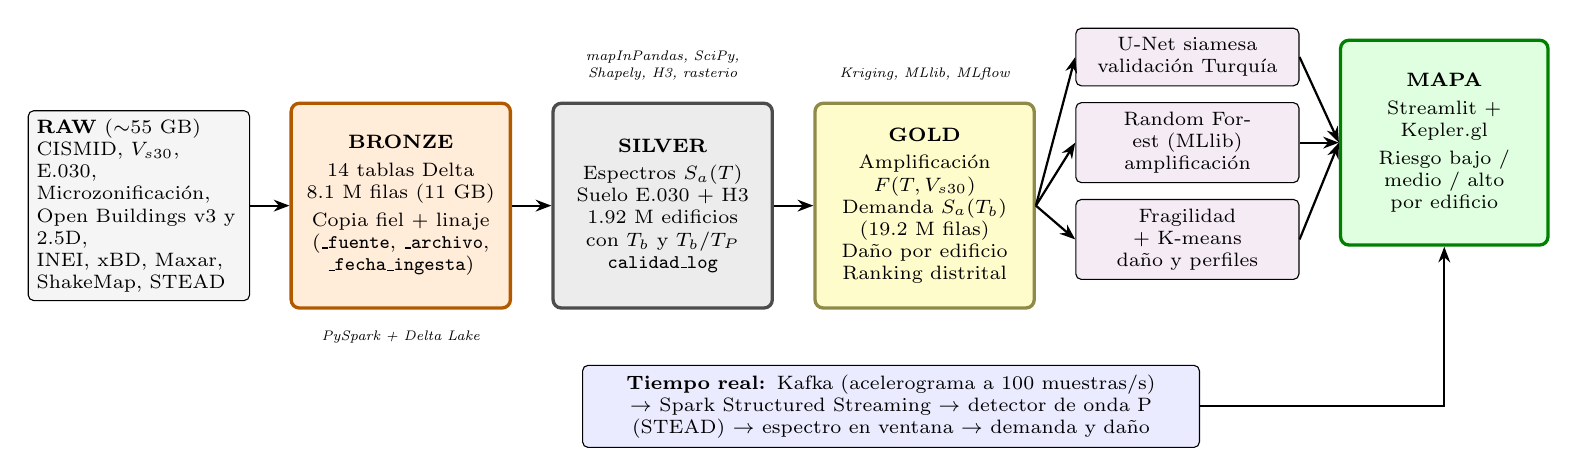
\begin{tikzpicture}[
  font=\scriptsize,
  node distance=4mm and 5mm,
  capa/.style={draw, rounded corners=3pt, align=center, minimum height=2.6cm, text width=2.55cm, very thick},
  src/.style={draw, rounded corners=2pt, align=left, fill=gray!8, text width=2.6cm, inner sep=3pt},
  mod/.style={draw, rounded corners=2pt, align=center, fill=violet!8, text width=2.6cm, minimum height=7mm},
  flecha/.style={-{Stealth[length=2mm]}, thick}]
% Fuentes
\node[src] (raw) {\textbf{RAW} (${\sim}55$ GB)\\CISMID, $V_{s30}$, E.030,\\Microzonificación,\\Open Buildings v3 y 2.5D,\\INEI, xBD, Maxar,\\ShakeMap, STEAD};
% Capas
\node[capa, fill=orange!15, draw=orange!70!black, right=of raw] (bronze) {\textbf{BRONZE}\\[2pt]14 tablas Delta\\8.1 M filas (11 GB)\\[2pt]Copia fiel + linaje\\(\texttt{\_fuente}, \texttt{\_archivo},\\\texttt{\_fecha\_ingesta})};
\node[capa, fill=gray!15, draw=gray!60!black, right=of bronze] (silver) {\textbf{SILVER}\\[2pt]Espectros $S_a(T)$\\Suelo E.030 + H3\\1.92 M edificios\\con $T_b$ y $T_b/T_P$\\\texttt{calidad\_log}};
\node[capa, fill=yellow!20, draw=yellow!50!black, right=of silver] (gold) {\textbf{GOLD}\\[2pt]Amplificación $F(T,V_{s30})$\\Demanda $S_a(T_b)$\\(19.2 M filas)\\Daño por edificio\\Ranking distrital};
% Modelos
\node[mod, right=of gold, yshift=8mm] (m1) {Random Forest (MLlib)\\amplificación};
\node[mod, below=2mm of m1] (m2) {Fragilidad + K-means\\daño y perfiles};
\node[mod, above=2mm of m1] (m0) {U-Net siamesa\\validación Turquía};
% Salida
\node[draw, rounded corners=3pt, fill=green!12, draw=green!50!black, very thick, align=center, text width=2.4cm, minimum height=2.6cm, right=of m1] (mapa) {\textbf{MAPA}\\[2pt]Streamlit +\\Kepler.gl\\[2pt]Riesgo bajo /\\medio / alto\\por edificio};
% Streaming
\node[draw, rounded corners=2pt, fill=blue!8, align=center, text width=7.6cm, below=7mm of silver, xshift=2.9cm] (stream) {\textbf{Tiempo real:} Kafka (acelerograma a 100 muestras/s) $\rightarrow$ Spark Structured Streaming $\rightarrow$ detector de onda P (STEAD) $\rightarrow$ espectro en ventana $\rightarrow$ demanda y daño};
% Flechas
\draw[flecha] (raw) -- (bronze);
\draw[flecha] (bronze) -- (silver);
\draw[flecha] (silver) -- (gold);
\draw[flecha] (gold.east) -- (m1.west);
\draw[flecha] (gold.east) -- (m2.west);
\draw[flecha] (gold.east) -- (m0.west);
\draw[flecha] (m1.east) -- (mapa.west);
\draw[flecha] (m2.east) -- (mapa.west);
\draw[flecha] (m0.east) -- (mapa.west);
\draw[flecha] (stream.east) -| (mapa.south);
% Tecnologías
\node[below=1.5mm of bronze, align=center, text width=2.6cm, font=\tiny\itshape] {PySpark + Delta Lake};
\node[above=1.5mm of silver, align=center, text width=2.8cm, font=\tiny\itshape] {mapInPandas, SciPy,\\Shapely, H3, rasterio};
\node[above=1.5mm of gold, align=center, text width=2.6cm, font=\tiny\itshape] {Kriging, MLlib, MLflow};
\end{tikzpicture}}
\caption{Arquitectura propuesta: lakehouse medallón en Apache Spark y Delta Lake, modelos analíticos, flujo en tiempo real y visualización.}
\label{fig:arquitectura}
\fuente{Elaboración propia.}
\end{figure*}

\begin{table}[!t]
\centering
\caption{Tecnologías de Big Data del proyecto}
\label{tab:tecnologias}
\footnotesize
\renewcommand{\arraystretch}{1.12}
\begin{tabularx}{\columnwidth}{>{\raggedright\arraybackslash}p{2.0cm} Y}
\toprule
\textbf{Tecnología} & \textbf{Uso} \\
\midrule
Apache Spark 4.2 (PySpark) & Motor de procesamiento distribuido de las tres capas \cite{zaharia2016spark}. \\
Delta Lake 4.4 & Formato de tablas ACID y versionadas del lakehouse \cite{armbrust2020delta}. \\
Pandas UDF (\texttt{mapInPandas}) + SciPy & Procesamiento paralelo de señales: filtrado y espectros. \\
Shapely (STRtree) + H3 & Cruces espaciales distribuidos (\emph{point-in-polygon}) e indexación hexagonal. \\
rasterio & Lectura remota de rásters de altura y $\vs$. \\
Spark MLlib & Random Forest de amplificación y K-means \cite{meng2016mllib}. \\
PyTorch & U-Net siamesa de daño y detector de onda P. \\
MLflow & Registro de experimentos, métricas y modelos. \\
Apache Kafka + Spark Structured Streaming & Ingesta y procesamiento en tiempo real \cite{kreps2011kafka}. \\
Streamlit + Kepler.gl & Tablero y mapa geoespacial interactivo. \\
\bottomrule
\end{tabularx}
\end{table}

El entorno de ejecución es un equipo con Windows~11, 16~GB de RAM y 16 núcleos lógicos, donde Spark se ejecuta en modo local (\texttt{local[4]}, 4~GB para el \emph{driver}). Las tablas Delta se almacenan por ruta en \texttt{lakehouse/bronze} y \texttt{lakehouse/silver}. La arquitectura es portable a un clúster o a la nube sin modificar el código.

\subsection{Capa Bronze: ingesta}
Cada fuente se carga como tabla Delta sin modificar su contenido, agregando columnas de linaje: \texttt{\_fuente}, \texttt{\_archivo} y \texttt{\_fecha\_ingesta}. De las imágenes y rásters pesados (xBD, Maxar, alturas y HDF5) solo se registran rutas y metadatos, sin copiar los píxeles a las tablas. Se construyeron 14 tablas con unos 8.1 millones de filas (11~GB) en aproximadamente 6~minutos. Entre los problemas resueltos destacan tres formatos de cabecera distintos en los acelerogramas del CISMID, archivos en codificación Latin-1, filas con saltos de línea en los metadatos de STEAD y la preservación del cero inicial de los identificadores \emph{quadkey} de Maxar.

\subsection{Capa Silver: limpieza y variables físicas}
\textbf{a) Ondas.} Cada acelerograma se procesa en paralelo con \texttt{mapInPandas}: corrección de línea base, ventana de Tukey del 5\,\%, filtro Butterworth pasa-banda de 0.1 a 25~Hz (orden 4, fase cero) y conversión de cm/s$^2$ a $g$. Luego se calculan $PGA$, $PGV$ y $S_a(T)$ en 50 periodos logarítmicamente espaciados entre 0.05 y 4~s, con el método exacto de Nigam y Jennings \cite{nigam1969} (validado contra integración de Newmark, con diferencias menores a 0.05\,\%). Las dos componentes horizontales se combinan con la media geométrica, $S_a^{GEO}=\sqrt{S_a^{EW}\,S_a^{NS}}$, y el periodo predominante se toma en el máximo del espectro. El resultado son las tablas \texttt{ondas\_registros} (137 filas) y \texttt{espectros} (27\,400 filas). La Tabla~\ref{tab:eventos} resume los cinco sismos.

\begin{table}[!t]
\centering
\caption{Sismos registrados en Lima y Callao (capa Silver)}
\label{tab:eventos}
\footnotesize
\setlength{\tabcolsep}{3.5pt}
\begin{tabular}{l c c c c}
\toprule
\textbf{Evento} & \textbf{Est.} & \makecell{\textbf{PGA}\\\textbf{máx. (g)}} & \makecell{\textbf{Dist.}\\\textbf{mín. (km)}} & \makecell{\textbf{$T_p$}\\\textbf{med. (s)}} \\
\midrule
Pisco 2007, $M_w$7.9 & 3 & 0.100 & 181 & 0.27 \\
Callao 2021, M5.2 & 32 & 0.090 & 77 & 0.07 \\
Lima 2022, M5.6 & 32 & 0.203 & 117 & 0.08 \\
Callao 2025, M6.1 & 32 & 0.304 & 57 & 0.13 \\
Ica 2026, M6.1 & 38 & 0.017 & 268 & 0.15 \\
\bottomrule
\end{tabular}
\end{table}

\textbf{b) Territorio.} Se filtran los 49 distritos de Lima y Callao. Cada píxel de $\vs$ recibe su perfil E.030 (S0: $>1500$, S1: 500--1500, S2: 180--500 y S3: $<180$~m/s), su factor $S$, sus periodos $T_P$ y $T_L$ y una celda H3. Las edificaciones pasan por un embudo de calidad (Tabla~\ref{tab:embudo}): recorte por rectángulo, \emph{point-in-polygon} con los 49 distritos mediante Shapely STRtree dentro de \texttt{mapInPandas}, filtro de confianza $\geq 0.75$ y eliminación de duplicados. A cada edificio se le asigna su celda H3 (resoluciones 9 y 8), su suelo y su altura 2.5D, leída en el centroide o, si falta, como el máximo en una ventana de $3\times3$ píxeles. Con la Ec.~\eqref{eq:tb} se obtienen $N$, $T_b$ y $T_b/T_P$. Además, se extraen del texto de los PDF las descripciones de las zonas I--V y 23 rangos de periodo predominante citados por la microzonificación.

\begin{table}[!t]
\centering
\caption{Embudo de calidad de las edificaciones}
\label{tab:embudo}
\footnotesize
\begin{tabular}{l r}
\toprule
\textbf{Etapa} & \textbf{Edificaciones} \\
\midrule
Tesela completa (Bronze) & 7\,219\,950 \\
Dentro del rectángulo de Lima & 3\,198\,445 \\
Dentro de los 49 distritos & 3\,124\,896 \\
Confianza $\geq 0.75$ y sin duplicados & \textbf{1\,921\,174} \\
\quad con altura en el centroide & 1\,718\,102 \\
\quad con altura por ventana $3\times3$ & 50\,131 \\
\quad sin altura (1 piso imputado) & 152\,941 \\
\bottomrule
\end{tabular}
\end{table}

\textbf{c) Validación.} Se prepara \texttt{xbd\_escenas} (conteo de píxeles por clase de daño en 8\,043 escenas, leyendo solo las máscaras), \texttt{maxar\_pares} (5 pares emparejados por \emph{quadkey} y fecha), \texttt{shakemap\_turquia} (intensidades convertidas a $g$) y \texttt{stead\_trazas} (llegadas P y S y relación señal/ruido de 200\,000 trazas).

\textbf{d) Control de calidad.} Toda fila descartada, imputada o fuera de alcance se registra en \texttt{calidad\_log} con la regla aplicada y su motivo (1.36 millones de registros), lo que garantiza la trazabilidad del proceso.

\subsection{Capa Gold y modelos analíticos}
\textbf{Paso 1. Amplificación del suelo medida con las ondas de Lima.} Para cada sismo se elige una estación de referencia sobre suelo firme (mayor $\vs$) y se calcula el cociente espectral de cada estación, corregido por la diferencia de distancia hipocentral $R$:
\begin{equation}
F_{obs}(T)=\frac{S_a^{est}(T)}{S_a^{ref}(T)}\cdot\frac{R_{est}}{R_{ref}}.
\label{eq:cociente}
\end{equation}
Con unas 6\,850 observaciones se entrena un \textbf{Random Forest de regresión} \cite{breiman2001rf} en Spark MLlib que estima $\ln F=f(T,\vs,\ldots)$, validado con la estrategia de dejar un evento fuera. El modelo se contrasta con los factores $S$ de la E.030 y con los periodos de la microzonificación.

\textbf{Paso 2. Demanda sísmica en cada edificación.} El efecto del suelo se retira en las estaciones para obtener el movimiento en roca, se interpola mediante \emph{kriging} ordinario a las celdas H3 de resolución 8 (unas 4\,000 en Lima) y se vuelve a amplificar con el suelo de cada edificio:
\begin{equation}
\begin{aligned}
S_a^{roca}(T)&=S_a^{est}(T)\,/\,F(T,V_{s30}^{est}),\\
S_a^{sitio}(T)&=S_a^{roca}(T)\,F(T,V_{s30}^{b}).
\end{aligned}
\label{eq:demanda}
\end{equation}
La demanda $S_a(T_b)$ se obtiene interpolando en $\log T$. Se evalúan 10 escenarios: los 5 sismos registrados y esos mismos espectros escalados al sismo de diseño de la E.030 con $k=0.45\,g/PGA_{roca}$. El volumen resultante es de $1.92\text{ M}\times 10=19.2$ millones de filas (unos 960 millones de valores con el espectro completo), lo que justifica el procesamiento distribuido.

\textbf{Paso 3. Daño y nivel de riesgo.} A cada edificación se asigna una tipología (albañilería confinada, adobe o concreto armado) según su zona y número de pisos, y se aplican \textbf{curvas de fragilidad lognormales} con parámetros de la literatura para Sudamérica \cite{villarvega2017}:
\begin{equation}
P\!\left(DS\geq ds \mid S_a(T_b)\right)=\Phi\!\left(\frac{\ln\!\left(S_a(T_b)/\theta_{ds}\right)}{\beta_{ds}}\right),
\label{eq:fragilidad}
\end{equation}
donde $\theta_{ds}$ es la mediana y $\beta_{ds}$ la dispersión del estado de daño $ds$ (leve, moderado, severo o colapso). La probabilidad de cada estado se obtiene por diferencia de curvas consecutivas. El nivel de riesgo se define como \emph{bajo} si $P(DS\geq\text{moderado})<0.2$, \emph{medio} si está entre 0.2 y 0.5, y \emph{alto} si es mayor o igual a 0.5; estos umbrales se calibrarán en la validación. Finalmente, \textbf{K-means} sobre $\big(S_a(T_b),\,T_b/T_P,\,\vs,\,N\big)$ agrupa las edificaciones en perfiles de riesgo (con $k$ elegido por el coeficiente de silueta), y los resultados se agregan por distrito y por hexágono H3.

\subsection{Validación con un sismo real}
Para comprobar la cadena \emph{onda $\rightarrow$ suelo $\rightarrow$ demanda $\rightarrow$ daño}, se usa el sismo de Turquía de 2023, donde el daño sí fue observado. Una \textbf{U-Net siamesa} \cite{ronneberger2015unet} entrenada con xBD detecta el daño en los 5 pares Maxar, recortados en ventanas de $1024\times1024$ píxeles. En paralelo, se aplican los pasos 2 y 3 en esas zonas usando el ShakeMap como onda. El daño predicho se compara con el observado mediante la matriz de confusión, el F1 por clase y el \emph{recall} de colapso. El detector se evalúa con la métrica de xView2: $0.3\,F1_{loc}+0.7\,F1_{daño}$.

\subsection{Procesamiento en tiempo real}
Un productor de \textbf{Apache Kafka} reproduce un acelerograma del CISMID a 100 muestras por segundo. \textbf{Spark Structured Streaming} lo consume en ventanas deslizantes de 4~s cada 1~s y aplica un detector de onda P entrenado con STEAD (GBT en MLlib o CNN 1D). Al detectar la onda P, calcula el espectro de la ventana, recalcula la demanda y el daño, y actualiza el mapa.

\subsection{Visualización}
Un tablero en \textbf{Streamlit} con \textbf{Kepler.gl} muestra cada edificación coloreada por su nivel de riesgo, los hexágonos H3, el ranking de distritos, un selector de escenarios y capas de suelo y resonancia.

\subsection{Modelos y métricas}
La Tabla~\ref{tab:modelos} resume los modelos, sus datos de entrada y sus métricas de evaluación.

\begin{table}[!t]
\centering
\caption{Modelos, datos y métricas}
\label{tab:modelos}
\footnotesize
\renewcommand{\arraystretch}{1.12}
\begin{tabularx}{\columnwidth}{>{\raggedright\arraybackslash}p{1.65cm} >{\raggedright\arraybackslash}p{1.75cm} Y}
\toprule
\textbf{Modelo} & \textbf{Algoritmo} & \textbf{Datos y métrica} \\
\midrule
Amplificación & Random Forest de regresión & Espectros CISMID + $\vs$; RMSE de $\ln F$ y comparación con E.030 \\
Daño & Curvas de fragilidad & Demanda + tipología; validación en Turquía (F1, \emph{recall} de colapso) \\
Perfiles de riesgo & K-means & Demanda, suelo y pisos; coeficiente de silueta \\
Detector de daño & U-Net siamesa & xBD $\rightarrow$ Maxar; F1 de xView2 \\
Onda P & GBT / CNN 1D & STEAD; precisión, \emph{recall} y error en segundos \\
\bottomrule
\end{tabularx}
\end{table}

\subsection{Las 5V del Big Data}
La Tabla~\ref{tab:5v} muestra cómo el proyecto responde a las cinco dimensiones del Big Data.

\begin{table}[!t]
\centering
\caption{Las 5V del Big Data en el proyecto}
\label{tab:5v}
\footnotesize
\renewcommand{\arraystretch}{1.12}
\begin{tabularx}{\columnwidth}{>{\raggedright\arraybackslash}p{1.45cm} Y}
\toprule
\textbf{V} & \textbf{Evidencia} \\
\midrule
Volumen & ${\sim}55$~GB crudos; 7.2 M edificaciones; 19.2 M filas de demanda (${\sim}960$ M valores). \\
Velocidad & Kafka + Spark Structured Streaming a 100 muestras/s. \\
Variedad & Texto, imágenes, netCDF, GeoTIFF, CSV, GeoJSON, XML, PDF y HDF5. \\
Veracidad & Linaje, \texttt{calidad\_log} (1.36 M filas), espectro validado contra Newmark, contraste con E.030 y Turquía. \\
Valor & Mapa de edificaciones en mayor riesgo y ranking distrital para la gestión del riesgo. \\
\bottomrule
\end{tabularx}
\end{table}

\subsection{Limitaciones}
\begin{itemize}
  \item Los sismos registrados en Lima son moderados ($PGA\leq0.30\,g$); por ello se escalan al sismo de diseño.
  \item El $\vs$ del USGS, derivado de la pendiente topográfica, no identifica suelos S3 en Lima; se corregirá con la microzonificación digitalizada.
  \item La altura 2.5D tiene 4~m de resolución efectiva y el 8\,\% de las edificaciones no tiene altura (se imputa 1 piso).
  \item La tipología constructiva se asume por zona, ya que no existe un catastro abierto, y $T_b=0.1N$ es una aproximación normativa.
  \item La validación usa un sismo cortical (Turquía), mientras que el esperado en Lima es de subducción, y xBD contiene pocas escenas de sismo (193).
\end{itemize}

% =====================================================================
\section{Conclusiones}\label{sec:conclusiones}
% =====================================================================
El estado del arte muestra que las imágenes satelitales permiten caracterizar edificaciones y detectar daño de forma automática \cite{carpanese2023,gupta2019xbd}, e incluso estimar la vulnerabilidad sísmica por píxel \cite{fan2021plsv}, y que las arquitecturas de Big Data con Kafka y Spark procesan formas de onda a gran escala y en tiempo real \cite{zhu2022quakeflow,li2022yangbi,xiao2026edge}. Sin embargo, estos enfoques no integran la respuesta del suelo ni la resonancia de cada edificio para anticipar el daño.

La propuesta combina ambas líneas en un lakehouse medallón sobre Apache Spark y Delta Lake, que ya integra 11 fuentes heterogéneas y procesa 1.92 millones de edificaciones de Lima con su suelo y su periodo de vibración. Su principal aporte es medir la amplificación del suelo con las propias ondas registradas en Lima y llevar la demanda sísmica hasta cada edificio, para producir un mapa de riesgo bajo, medio y alto que oriente la gestión del riesgo de desastres en la ciudad.

% =====================================================================
\begin{thebibliography}{99}
\footnotesize

\bibitem{tavera2024}
% [Completar título exacto del informe citado]
H. Tavera y Mamani, ``Informe técnico del Instituto Geofísico del Perú,'' Instituto Geofísico del Perú, Lima, Perú, 2024.

\bibitem{inei2025}
Instituto Nacional de Estadística e Informática (INEI), ``Lima supera los 10 millones 400 mil habitantes,'' nota de prensa, 2025. [En línea]. Disponible: \url{https://www.gob.pe/institucion/inei/noticias/1092367-lima-supera-los-10-millones-400-mil-habitantes}

\bibitem{tavera2025}
H. Tavera, ``Sismo del Callao del 15 de junio, 2025 (M6.1) y niveles de sacudimiento del suelo,'' Instituto Geofísico del Perú, Lima, Perú, jun. 2025. [En línea]. Disponible: \url{https://repositorio.igp.gob.pe}

\bibitem{igp_saspe}
Instituto Geofísico del Perú (IGP), ``Sistema de Alerta Sísmica Peruano (SASPe),'' s.f. [En línea]. Disponible: \url{https://www.igp.gob.pe}

\bibitem{carpanese2023}
P. Carpanese, M. Donà y F. da Porto, ``Automatic identification of residential building features using machine learning techniques,'' \emph{Procedia Structural Integrity}, vol. 44, pp. 1980--1987, 2023, doi: 10.1016/j.prostr.2023.01.253.

\bibitem{fan2021plsv}
X. Fan, G. Nie, C. Xia y J. Zhou, ``Estimation of pixel-level seismic vulnerability of the building environment based on mid-resolution optical remote sensing images,'' \emph{International Journal of Applied Earth Observation and Geoinformation}, vol. 101, art. 102339, 2021, doi: 10.1016/j.jag.2021.102339.

\bibitem{gupta2019xbd}
R. Gupta \emph{et al.}, ``xBD: A dataset for assessing building damage from satellite imagery,'' \emph{arXiv preprint} arXiv:1911.09296, 2019.

\bibitem{zhu2022quakeflow}
W. Zhu, A. B. Hou, R. Yang, A. Datta, S. M. Mousavi, W. L. Ellsworth y G. C. Beroza, ``QuakeFlow: A scalable machine-learning-based earthquake monitoring workflow with cloud computing,'' \emph{Geophysical Journal International}, vol. 232, no. 1, pp. 684--693, 2022, doi: 10.1093/gji/ggac355.

\bibitem{li2022yangbi}
J. Li \emph{et al.}, ``A real-time AI-assisted seismic monitoring system based on new nodal stations with 4G telemetry and its application in the Yangbi MS 6.4 aftershock monitoring in southwest China,'' \emph{Earthquake Research Advances}, 2022.

\bibitem{xiao2026edge}
% [Completar autores, revista, volumen y DOI]
Xiao \emph{et al.}, ``Edge seismic phase picking: Model distillation for multimodal early-warning systems,'' 2026.

\bibitem{e030}
Ministerio de Vivienda, Construcción y Saneamiento, ``Norma Técnica E.030 Diseño Sismorresistente,'' D.S. N.\textsuperscript{o} 003-2016-VIVIENDA, modificada por R.M. N.\textsuperscript{o} 355-2018-VIVIENDA, Lima, Perú, 2018.

\bibitem{cismid_redacis}
Centro Peruano Japonés de Investigaciones Sísmicas y Mitigación de Desastres (CISMID-FIC-UNI), ``Red Acelerográfica del CISMID (REDACIS),'' 2026. [En línea]. Disponible: \url{https://www.cismid.uni.edu.pe/ceois/redacis/red/}

\bibitem{heath2020vs30}
D. C. Heath, D. J. Wald, C. B. Worden, E. M. Thompson y G. M. Smoczyk, ``A global hybrid $V_{S30}$ map with a topographic slope-based default and regional map insets,'' \emph{Earthquake Spectra}, vol. 36, no. 3, pp. 1570--1584, 2020, doi: 10.1177/8755293020911137.

\bibitem{cismid_microzon}
CISMID-FIC-UNI, ``Estudios de microzonificación sísmica de los distritos de Cercado de Lima, Comas, La Molina y Villa El Salvador,'' SIGRID-CENEPRED, 2010--2013. [En línea]. Disponible: \url{https://sigrid.cenepred.gob.pe}

\bibitem{sirko2021openbuildings}
W. Sirko \emph{et al.}, ``Continental-scale building detection from high resolution satellite imagery,'' \emph{arXiv preprint} arXiv:2107.12283, 2021.

\bibitem{sirko2023temporal}
W. Sirko \emph{et al.}, ``High-resolution building and road detection from Sentinel-2,'' \emph{arXiv preprint} arXiv:2310.11622, 2023.

\bibitem{peru_geojson}
juaneladio, ``peru-geojson: Límites políticos del Perú (fuente: INEI),'' repositorio GitHub. [En línea]. Disponible: \url{https://github.com/juaneladio/peru-geojson}

\bibitem{maxar_open}
Maxar Technologies, ``Maxar Open Data Program: Kahramanmaraş, Turkey earthquake,'' 2023. [En línea]. Disponible: \url{https://www.maxar.com/open-data}

\bibitem{usgs_shakemap}
U.S. Geological Survey, ``M 7.8 -- Pazarcık earthquake, Kahramanmaraş earthquake sequence (us6000jllz): ShakeMap,'' 2023. [En línea]. Disponible: \url{https://earthquake.usgs.gov/earthquakes/eventpage/us6000jllz/shakemap}

\bibitem{mousavi2019stead}
S. M. Mousavi, Y. Sheng, W. Zhu y G. C. Beroza, ``STanford EArthquake Dataset (STEAD): A global data set of seismic signals for AI,'' \emph{IEEE Access}, vol. 7, pp. 179464--179476, 2019, doi: 10.1109/ACCESS.2019.2947848.

\bibitem{zaharia2016spark}
M. Zaharia \emph{et al.}, ``Apache Spark: A unified engine for big data processing,'' \emph{Communications of the ACM}, vol. 59, no. 11, pp. 56--65, 2016.

\bibitem{armbrust2020delta}
M. Armbrust \emph{et al.}, ``Delta Lake: High-performance ACID table storage over cloud object stores,'' \emph{Proceedings of the VLDB Endowment}, vol. 13, no. 12, pp. 3411--3424, 2020.

\bibitem{meng2016mllib}
X. Meng \emph{et al.}, ``MLlib: Machine learning in Apache Spark,'' \emph{Journal of Machine Learning Research}, vol. 17, no. 34, pp. 1--7, 2016.

\bibitem{kreps2011kafka}
J. Kreps, N. Narkhede y J. Rao, ``Kafka: A distributed messaging system for log processing,'' en \emph{Proc. NetDB Workshop}, 2011.

\bibitem{nigam1969}
N. C. Nigam y P. C. Jennings, ``Calculation of response spectra from strong-motion earthquake records,'' \emph{Bulletin of the Seismological Society of America}, vol. 59, no. 2, pp. 909--922, 1969.

\bibitem{breiman2001rf}
L. Breiman, ``Random forests,'' \emph{Machine Learning}, vol. 45, no. 1, pp. 5--32, 2001.

\bibitem{villarvega2017}
M. Villar-Vega \emph{et al.}, ``Development of a fragility model for the residential building stock in South America,'' \emph{Earthquake Spectra}, vol. 33, no. 2, pp. 581--604, 2017.

\bibitem{ronneberger2015unet}
O. Ronneberger, P. Fischer y T. Brox, ``U-Net: Convolutional networks for biomedical image segmentation,'' en \emph{Medical Image Computing and Computer-Assisted Intervention (MICCAI)}, LNCS, vol. 9351, 2015, pp. 234--241.

\end{thebibliography}

\end{document}
